\documentclass[manuscript,review,anonymous]{acmart}
\usepackage{caption}
\usepackage{subcaption}
\usepackage{hyperref}

% NOTE: Good things
%  - what is iterative prompting? "Like auto-complete but less limited" - hmm, maybe
%  - sell more main idea: can do much with very limited set of commands / via auto-complete
%  - paper is convincing in that this works for SQL-like queries (maybe not general purpose, but this is good)
%  - journalism is a good focus / but needs to deemphasize this a bit because of the study
%  - #1 Limited language for data exploration (what is included / excluded / essential / could be added)
%  - #2 Iterative prompting - what's new? people can get to all programs via '.' and up/down/enter.

% NOTE: Random
%  - How choices were made?
%  - Terminology: data analysis / data exploration / data visualization - what is the goal of the system? (fair enough)
%    (it's not about writing charts - just about getting the right data - we have limited charting functionality,
%     one could integrate with Vega, or do future work based on iterative prompting)
%  - Technical details - you can only create valid programs!! (it's contextual)
%  - Minor: what was "demo" at the start of a session
%  - Table 1 vs. Table 2 numbers of participants
%  - What data quality is needed to make this work?
%  - "Magic Escalator of Knowledge" - remove bs?
%  - Clarify how we support 3D cubes (no unified API); mention "done by intern in X weeks"

% TODO Study improvements
% - The questionaire needs a bit more introduction when you present  the study.
% - When looking at the data for the questionaire, it seems somewhat inconclusive
%    as all the values lie around 2.5.  I think this warrants a bit more discussion.
% - Connected to this, I would recommend to highlight the successes of the study a bit more in the
%     discussion and  presentation of the results. You actually got non-programmers to do
%     sophisticated queries! That you didn't get support for all RQs is perhaps more a result of being quite  ambitious!

% TODO
%   - SAY SOMEWHERE: choose function *and* specify arguments via auto-complete
%   - ADD: table of all available operations? (shorten introduction)

% NOTE: Contribution
%  - What is the exact goal? (so that it can be compared with R, Python, Vega-Lite, Tableau)
%  - How the design goals were generated? (not by talking to journalists)
%  - "notebooks are messy" - not arguing we can fix that

% NOTE: Motivation
% - what if you could write the whole program using auto-complete?



% extend autocomplete into a full-blown interactive programming mechanism
% and show that it is viable for small programming tasks like data exploration
%
% --- remove some of the motivation (makes ppl ask bad questions)



%
% Iterative prompting - should we call it expression completion
% (is it more general result, or is it a new thing?)
% -> emphasize the why this is called differently paragraph
%
% Explain type providers a bit more (we say what it does, but not much about what
% it is - give dynamic typing in a static language)
%
% The 'then' operation was mysterious - can we add one line explanation to the operations?
% (yes we can and we should totally do that)
















% \usepackage{xspace}
\usepackage{fancyvrb}
% \usepackage{inconsolata}
\usepackage{xcolor}
% \usepackage{tikz}
% \newcommand*{\priority}[1]{\begin{tikzpicture}[scale=0.12]%
%     \draw (0,0) circle (1);
%     \fill[fill opacity=1,fill=black] (0,0) -- (90:1) arc (90:90-#1*3.6:1) -- cycle;
%     \end{tikzpicture}}
% \newcommand*{\priorityc}[1]{
% \resizebox{0.8em}{0.8em}{
%   {\protect\tikz{ \protect
%     \draw[line width=1mm, black] (0,0) circle (1); \fill[fill opacity=1,fill=black] (0,0) -- (90:1) arc (90:90-#1*3.6:1) -- cycle;
%     } }}}
%
\definecolor{kvdclr}{rgb}{0.3,0.0,0.8}
\DefineVerbatimEnvironment{thegamma}{Verbatim}{fontfamily=zi4,numbers=left,xleftmargin=6mm,fontsize=\small,commandchars=\\\{\}}
% %\newcommand{\kvd}[1]{\textcolor{kvdclr}{#1}}
\newcommand{\kvd}[1]{\textbf{#1}}
\newcommand{\ikvd}[1]{{\fontfamily{zi4}\selectfont\small #1}}
% \usepackage{balance}       % to better equalize the last page
% \usepackage{graphics}      % for EPS, load graphicx instead
% \usepackage[T1]{fontenc}   % for umlauts and other diaeresis
% \usepackage{txfonts}
% \usepackage{mathptmx}
% \usepackage[pdflang={en-US},pdftex]{hyperref}
% \usepackage{color}
% \usepackage{booktabs}
% \usepackage{textcomp}

\setcopyright{acmwhatever}
\copyrightyear{2020}
\acmYear{2020}
%\acmDOI{10.1145/1122445.1122456}
\acmConference[Woodstock '18]{Woodstock '18: ACM Symposium on Neural
  Gaze Detection}{June 03--05, 2018}{Woodstock, NY}
\acmBooktitle{Woodstock '18: ACM Symposium on Neural Gaze Detection,
  June 03--05, 2018, Woodstock, NY}
\acmPrice{15.00}
%\acmISBN{978-1-4503-XXXX-X/18/06}

\begin{document}
\title{The Gamma: Data Exploration through Iterative Prompting}

\author{Tomas Petricek}
\email{t.petricek@kent.ac.uk}
\affiliation{%
  \institution{University of Kent}
  \city{Canterbury, UK}
}
%\renewcommand{\shortauthors}{Trovato and Tobin, et al.}

\begin{abstract}
  Governments, non-profit organizations and citizen initiatives publish increasing amounts of
  data, but extracting insights from such data and presenting them to the public is hard.
  First, data comes in a variety of formats that each requires a different tool. Second, many
  data exploration tools do not reveal how a result was obtained, making it difficult to reproduce
  the results and check how they were obtained.
  %
  We contribute The Gamma, a novel data exploration environment for non-experts. The Gamma is based
  on a single interaction principle and using it results in transparent and reproducible scripts.
  This allows transfer of knowledge from one data source to another and
  learning from previously created data analyses. We evaluate the usability and learnability of
  The Gamma through a user study on non-technical employees of a research institute.
  %
  We argue that our approach allows journalists and the public to benefit from the rise
  of open data, by making data exploration easier, more transparent and more reproducible.

\end{abstract}

\begin{CCSXML}
<ccs2012>
   <concept>
       <concept_id>10003120.10003121.10003124</concept_id>
       <concept_desc>Human-centered computing~Interaction paradigms</concept_desc>
       <concept_significance>500</concept_significance>
       </concept>
   <concept>
       <concept_id>10011007.10011006.10011050.10011017</concept_id>
       <concept_desc>Software and its engineering~Domain specific languages</concept_desc>
       <concept_significance>300</concept_significance>
       </concept>
   <concept>
       <concept_id>10011007.10011006.10011066.10011069</concept_id>
       <concept_desc>Software and its engineering~Integrated and visual development environments</concept_desc>
       <concept_significance>500</concept_significance>
       </concept>
 </ccs2012>
\end{CCSXML}

\ccsdesc[500]{Human-centered computing~Interaction paradigms}
\ccsdesc[500]{Software and its engineering~Integrated and visual development environments}
\ccsdesc[300]{Software and its engineering~Domain specific languages}
\keywords{data exploration; end-user programming; data journalism; programming languages; type providers}

\maketitle

\begin{figure}
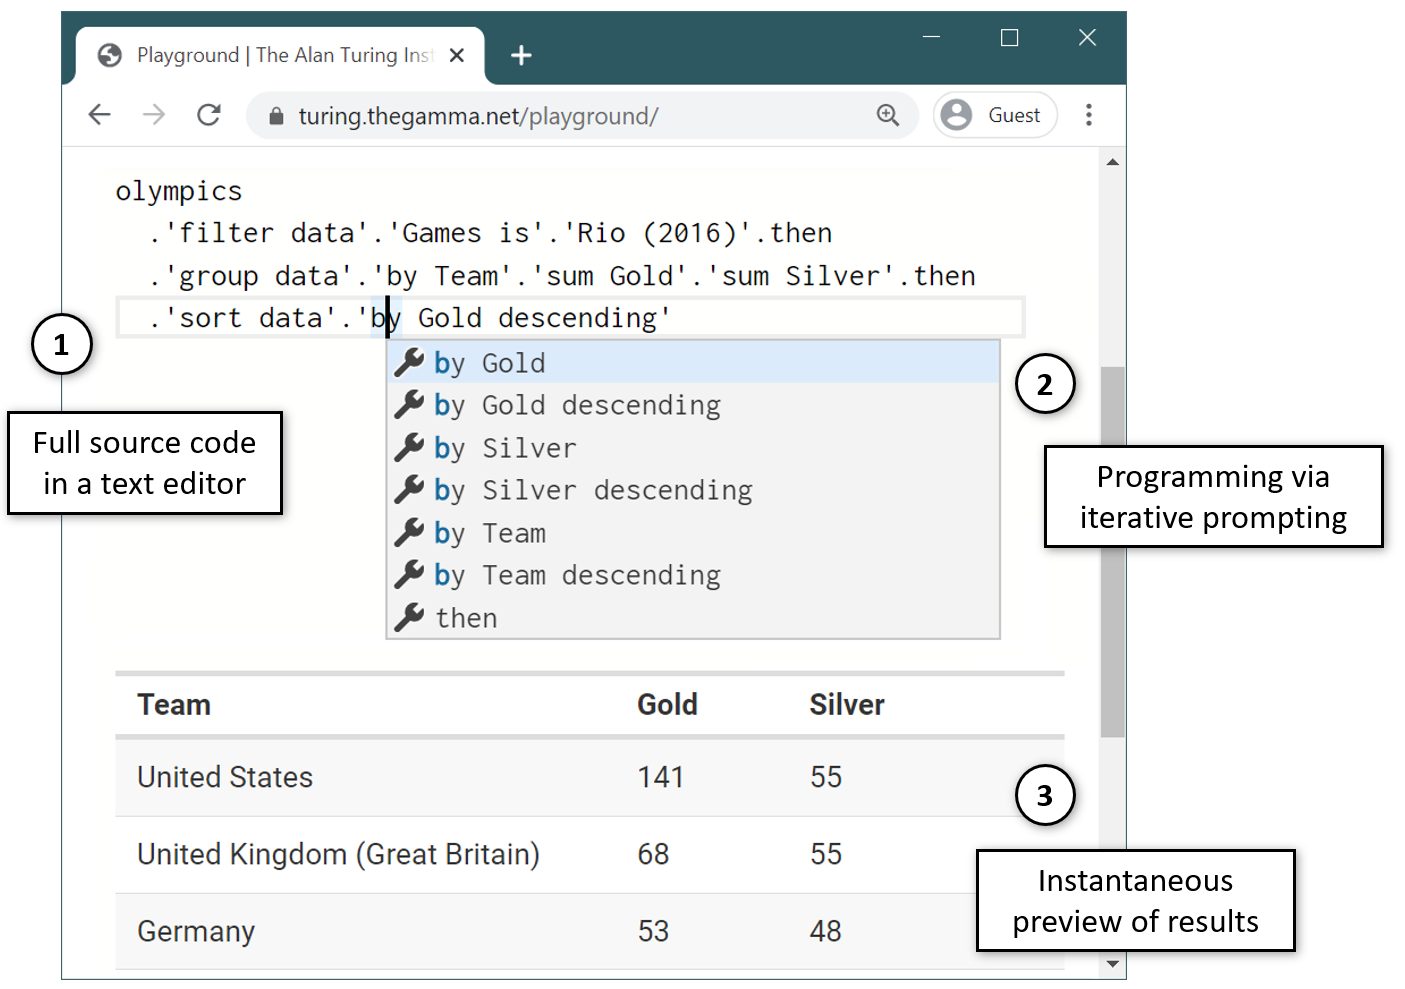
\includegraphics[width=.54\columnwidth]{figures/thegamma-annot}
\caption{Obtaining teams with the greatest number of gold medals from Rio 2016
Olympics with a reproducible The Gamma script (1), contextual iterative prompting mechainsm
offering ways of sorting the data (2) and an instant preview of results (3).}
\label{fig:thegamma}
\end{figure}

\section{Introduction}
Data science has more capabilities to help us understand the world than ever before, yet at the
same time post-truth politics and increasing public distrust in statistics makes data-driven insights
increasingly less relevant in public discourse~\cite{howstatslost}. To reverse this trend, we
need tools that let non-experts, including journalists and other information-literate citizens,
produce transparent, engaging data analyses that are easy to interpret without requiring expert
programming skill~\cite{ddj}. The design of such data exploration tool poses a unique mix of chellenges.
First, the tool needs to have a very low barrier to entry. Second, it needs to support a wide
range of data sources in a uniform way. Third, the resulting data analyses need to assist
readers in learning how to reproduce the work and verify the claims it makes.

We contribut The Gamma, a text-based data exploration environment for non-experts. The Gamma
is based on a single, easy to understand interaction principle and provides a uniform
access to a range of data sources including data tables, graph databases and data cubes.
The resulting analysis is a transparent script that can be followed to reproduce the
result from scratch. This allows learning from existing analyses and encourages readers
to engage with data.

\subsubsection*{Iterative Prompting}
The key idea in The Gamma, which we term the \emph{iterative prompting} principle, is that all
valid data exploration scripts can be constructed by repeatedly choosing from a list
of offered options. This way, non-programmers can write entire scripts through auto-complete,
without learning a programming language, but they still produce transparent and reproducible
source code. In other words, iterative prompting turns auto-complete from a programmer assistance
tool into a non-expert programming mechanism. A crucial feature is that iterative prompting
only offer operations that are valid in a given context and that it offer all such operations;
it is both correct and complete.

\subsubsection*{Data Exploration}
The Gamma focuses on data exploration of the kind illustrated in Figure~\ref{fig:thegamma}.
The user accesses data available in a structured format. They make several experiments to find an
interesting way of looking at the data, e.g.~by applying different aggregations or filters. They
may choose to view the results as a table or a basic chart before publishing their analysis. The
Gamma makes such simple programming with data simple enough for non-experts. Scraping and cleaning
of messy data or building rich data visualizations is outside of the scope of this paper, but
exposing those using the iterative prompting approach is an interesting future challenge.

\subsubsection*{Contributions}
The Gamma is available (non-anonymously) at \url{http://thegamma.net},
both as a JavaScript library and a hosted data exploration service. In this paper, we describe and
evaluate the design principles behind the project:

\begin{itemize}
\item We introduce the iterative prompting principle in The Gamma (Section~\ref{sec:overview})
  and show that it can be used for querying of distinct data sources including data tables, graph
  databases and data cubes (Section~\ref{sec:implementation}).

\item We show that iterative prompting is a complete and correct program construction method and
  consider how it lowers the barrier to entry and allows learning through examples, without
  expert guidance (Section~\ref{sec:design}).

\item We evaluate the system through a number of case studies (Section~\ref{sec:cases})
  and a user study (Section~\ref{sec:study}). Our study shows that non-programmers can use The Gamma
  to construct non-trivial data queries and ascertains the extent to which users can,
  (i) learn from examples and (ii)~transfer knowledge between tasks.
\end{itemize}


\section{Related Work}

The key contribution of our work is that it develops a new, fundamentally different, way of using the
established auto-completion mechanism. Unlike most past work dating back to Kaiser~\cite{assistants},
we do not view it as a programmer assistance tool, but as an interaction mechanism through which
non-experts can create entire programs. We build on recent research on information-rich
programming \cite{inforich} and aim to make those advances available to non-programmers
\cite{enduser,smallmatter}, in the context of data exploration as done, most notably, by
journalists \cite{ddj}. Our work features a novel combination of characteristics in that
the iterative prompting we develop (i) is centered around editing and understanding of program code,
(ii) its conceptual complexity is reduced to a single basic kind of interaction, yet (iii) it is
correct and complete in that it can be used to construct all meaningful programs.

\subsubsection*{Code Completion for Data Science}

A key component in The Gamma is the use of auto-complete for offering possible operations.
Our work follows type providers \cite{inforich,fsdata}, which integrate external data into a
static type system of F\#, allowing the use of auto-completion; for querying data tables, we utilize
the theory developed by Petricek \cite{dotdriven}. The key difference in our work is that The Gamma
can be used without a programming language expertise.

Most similar to our approach are tools that recommend scripts when users begin interacting
with data. Those based on machine learning code completion for domain-specific languages \cite{predictive,proactive}
differ in that they do not guarantee completeness, i.e.~the user cannot create all possible
scripts. Approaches based on natural language can effectively support data exploration
or visualization \cite{eviza,codemend}, but hide the structure of the underlying language and
require more than just selecting options. Conversational agents \cite{iris} improve on such work
in that they can provide more guidance. Code completion based on machine learning or statistical
methods \cite{mlcomplete,statcomplete} also exists for general-purpose programming languages used
by data scientists such as Python \cite{pythia}, providing assistance to expert programmers.
Finally, DS.js \cite{dsjs} is interesting in that it enables querying of data on the
web; it uses JavaScript with rich contextual code completion.

\subsubsection*{Notebooks and Business Intelligence Tools}

Notebooks such as Jupyter \cite{jupyter}, which allow combining source code with commentary and
visual outputs, are widely used by data scientists, but require expert programming skills.
The Gamma targets non-experts, but could be easily integrated with a multi-language notebook system
such as Wrattler \cite{wrattler}.

Spreadsheets and business intelligence tools \cite{tableau,powerbi} do
not involve programming, but require mastering a complex GUI. This is also the case
for other visual data analytics tools \cite{control,vizdom}. In contrast, The Gamma is
based on a single kind of interaction. Several visual systems \cite{potter,wrangler,lyra} record
interactions with the GUI as a script that can be seen and modified by the user.
Unlike in The Gamma, the source code does not guide the user in learning how to use the system.

\subsubsection*{Easier Programming Tools}
We aim to build an easy to use and learn programming system. Many approaches to this
goal have been tried. Victor \cite{learnable,principle} introduced design principles that
inspired many to build live programming systems \cite{review,liveroad,lighttable} that give
immediate feedback to help programmers understand how code relates to output and
exploratory systems \cite{variolite,exploratory} that assist with completing open-ended tasks.
A system combining textual language with visualization also exists for graph querying \cite{guess}.
To avoid difficulties with editing code as text, some systems use structured editors~\cite{structure-based,livenut,lamdu}.
In Subtext \cite{subtext,directprog} the language itself is co-designed with the editor to make
the interactions with code more natural. The Gamma is live in that our editor gives an instant
preview of the results.

Many systems simplify programming by designing high-level declarative abstractions,
e.g.~for interactive news articles \cite{idyll}, statistical analyses \cite{tea}
or interactive data visualization \cite{interactionviz,vegalite}. The Gamma uses
high-level abstractions for data querying, but designing high-level iterative prompting
abstractions for other tasks remains future work.

\subsubsection*{Programming without Writing Code}
There are two main approaches to programming where
the user does not write code. In programming by example \cite{byexample}, the user gives
examples of desired results. This has been used, e.g.~for specifying data transformations
in spreadsheets and data extraction \cite{spreadsheetpbe,flashextract}.
In direct manipulation \cite{direct}, a program is specified by directly interacting with the
output. This has been used in the visual domain \cite{sketchnsketch}, but also for data querying
\cite{dynamicq,vlang}. The VQE language~\cite{visage} also considers how to allow code reuse and
modification in this context. Direct manipulation can also support data exploration by letting
users partially edit queries,~e.g. by changing quantifiers as in DataPlay~\cite{dataplay}.

\subsubsection*{Guestures and Data Entry}
Although our focus is on program construction, our work can be positioned in the
broader context of input methods. Akin to Dasher \cite{dasher}, our system provides a way of
navigating through a complete space of options, while on-screen feedforward \cite{octopocus} allows
efficient selection in guesture-based interfaces. Those provide compelling alternatives to
auto-completion menus, although the efficiency of input methods is not an issue in programming.


\begin{figure}[b]
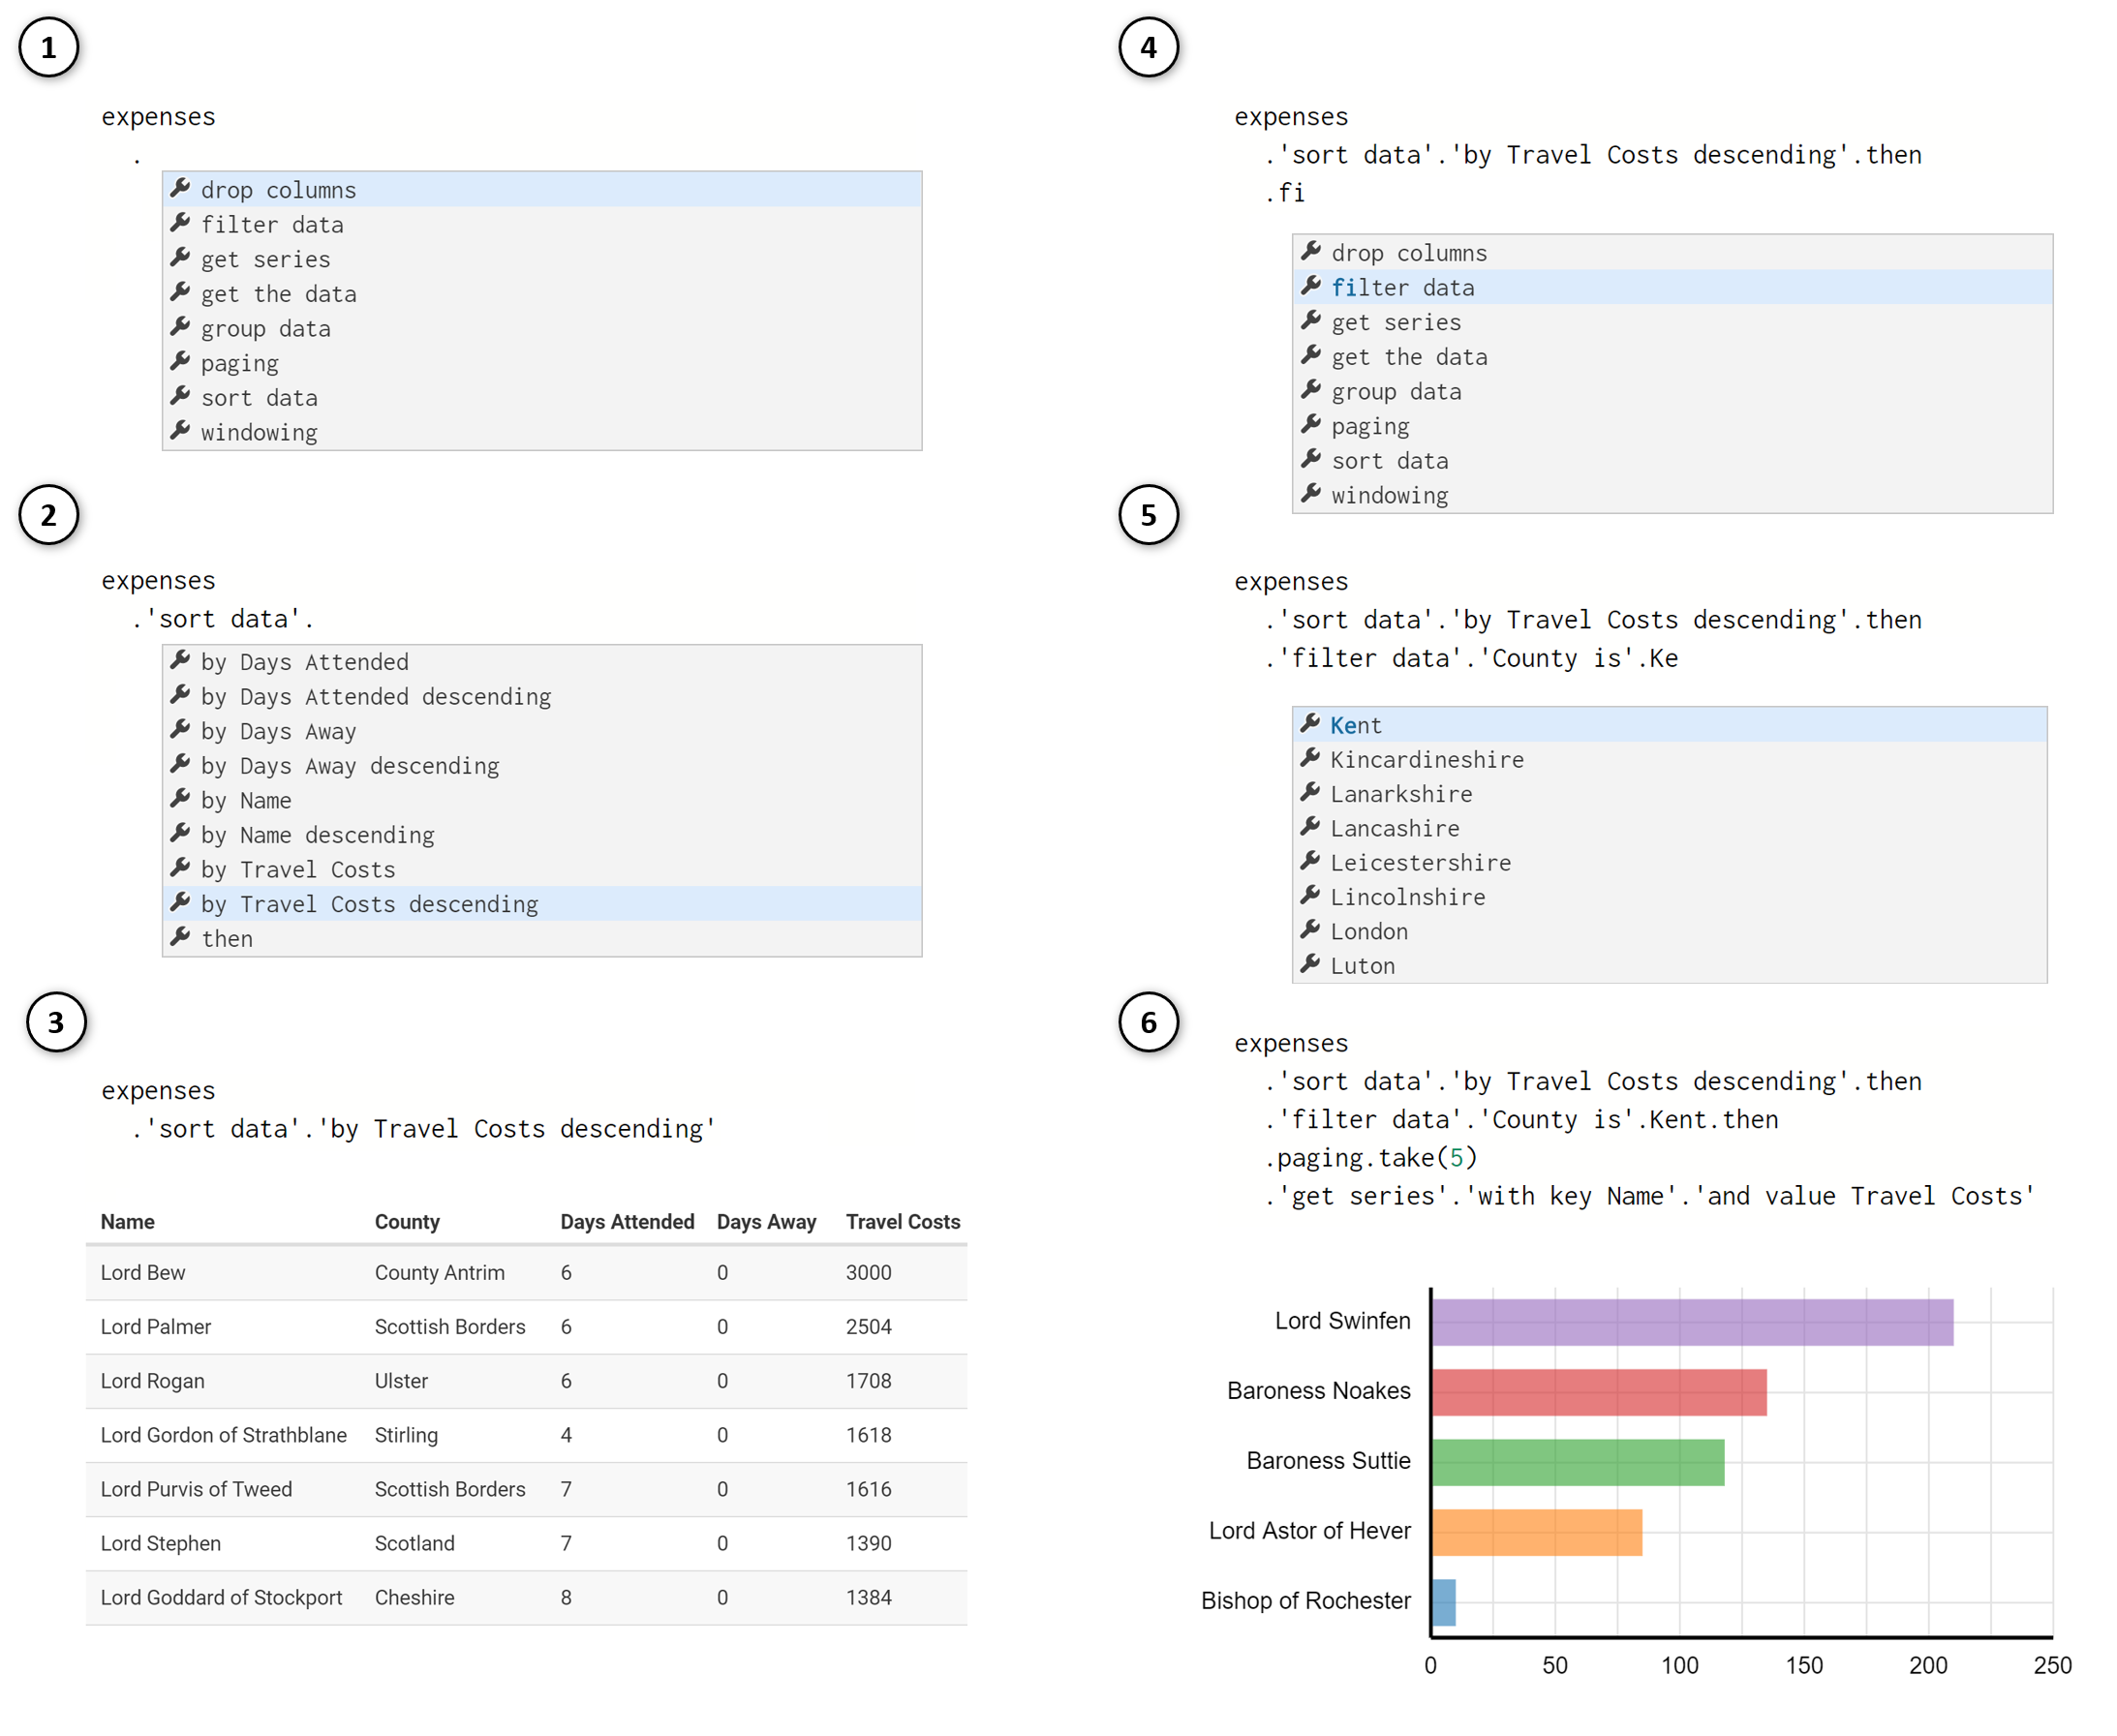
\includegraphics[width=1\columnwidth]{figures/thegamma-walk}
\caption{Constructing a script that charts the top 5 members of the House of Lords for Kent, based
on their travel costs.}
\label{fig:walkthrough}
\end{figure}

\section{Overview}
\label{sec:overview}

The review of related work suggests that there is an unexplored point in the design space of tools
for data exploration. Although various efforts make text-based programming easier, e.g. by providing
high-level declarative abstractions, most systems that target non-experts shy away from code, by using
either programming by example, natural language or graphical user interface. As spelled out in
Section~\ref{sec:design}, text-based programming has notable benefits for public-facing data analyses
such as learnability and transparency. Our work is thus motivated primarily by the question whether we
can make text-based programming easy enough for non-experts? The study presented in Section~\ref{sec:study}
shows that this is, indeed, possible at least for typical data querying tasks.
The Gamma consists of a programming language, a web-based coding environment and a number of type providers
that enable access to various kinds of data sources. It allows non-experts to create programs using the
\emph{iterative prompting} interaction principle -- by repeately selecting an item from an auto-complete list.
We start with a walkthrough of the system (Section~\ref{sec:overview-walk}), before looking at details of
The Gamma language (Section~\ref{sec:overview-lang}) and individual type providers (Section~\ref{sec:overview-tps}).

\subsection{Querying Travel Expenses}
\label{sec:overview-walk}

To introduce The Gamma, we walk through a simple problem that a local journalist might want to solve.
The UK government publishes travel expense claims by members of the House of Lords. We want to find
out which of the members representing the Kent county spend the most on travel.
The following shows a subset of the data:\footnote{Full data set has been obtained from
\url{https://www.parliament.uk/mps-lords-and-offices/members-allowances/house-of-lords/holallowances/} }

\begin{thegamma}
\textbf{Name, County, Days Attended, Days Away, Travel Costs}
Lord Adonis, London, 8, 0, 504
Baroness Afshar, Yorkshire, 2, 0, 0
Lord Alderdice, Oxfordshire, 3, 0, 114
Lord Alli, London, 5, 0, 0
\end{thegamma}
% Baroness Amos, London, 3, 0, 0

\noindent
The data is available as a CSV file. After the analyst imports the file through a web interface,
the environment is initialized with code that refers to the imported data as \ikvd{expenses}
and she starts exploring the data using the type provider for tabular data (Section~\ref{sec:overview-tps}),
following the steps illustrated in Figure~\ref{fig:walkthrough}:

\begin{enumerate}
\item The analyst types `.' (dot) to trigger auto-completion on \ikvd{expenses}. The type provider
  offers a list of operations that the analyst might want to perform such as grouping,
  filtering and sorting.

\item To find the House of Lords with the largest spending, the analyst chooses the
  \ikvd{sort data} operation. Next, she is offered a list of possible arguments based on the
  schema of the tabular data and chooses the desired one.

\item The Gamma evaluates the source code on-the-fly and shows a preview
  of results. After choosing the sorting key, the analyst sees a table with House of Lords members
  from more remote counties of the UK.

\item To finish specifying the (possibly compound) sorting key, the analyst chooses \ikvd{then}
  and is offered the same list of querying operations as in the first step. To obtain House
  members from Kent, she chooses \ikvd{filter data}. To navigate through the offered list more
  efficiently, she types first two characters of the name.

\item After selecting \ikvd{County is} to specify the desired type of condition, the analyst types
  `.' and is offered a list of options based on the values of the \ikvd{County} column in the
  source data set. She types \ikvd{Ke} and selects \ikvd{Kent}.

\item The analyst chooses \ikvd{then} and is,
  again, offered the list of querying operation. She uses \ikvd{paging} to get top 5 records,
  which requires typing \ikvd{5} as the argument. She then uses the \ikvd{get series} operation
  to obtain a data series associating travel expenses with a name, which is automatically
  visualized using a bar chart.
\end{enumerate}

\noindent
The constructed code is not unlike an SQL query, except that the whole script is constructed using
iterative prompting, by repeatedly selecting one of the offered members. Those represent both
operations, such as \ikvd{sort by} and arguments, such as \ikvd{Kent}. The only exception
is when the analyst needs to type the number \ikvd{5} to specify the number of items to take.

\subsection{The Gamma Programming Environment}
\label{sec:overview-lang}

The Gamma consists of a text-based programming language with a web-based coding environment,
based on the Monaco editor\footnote{For more information, see \url{https://microsoft.github.io/monaco-editor/}},
and type providers that provide access to data tables, graph databases and data cubes.

\subsubsection*{The Gamma Language}
A program in The Gamma is a sequence of commands. A command can be either a variable declaration
or an expression that evaluates to a value such as a data table or a chart.
An expression is a reference to a data source followed by a chain of member accesses.
A member can be either an ordinary member such as \ikvd{paging} or an operation which takes a
list of parameters enclosed in parentheses as in \ikvd{take(5)}. When the member name contains
non-alphanumerical characters it is  written in quotes such as \ikvd{\textquotesingle sort by\textquotesingle}.

The Gamma uses a type system to infer what members are available at a given point in a chain.
Each expression has a type with a list of members that, in turn, have their own types.
The types are not built-in, but are generated by type providers for individual data sources.
The programming environment for The Gamma is based on a text editor. When the user types `.'
the editor triggers auto-completion and retrives a list of available members based on the type
information. The programming environment evaluates scripts on-the-fly and shows a preview as
illustrated in Figure~\ref{fig:thegamma}.

\subsubsection*{Making Complex Things Possible}
As illustrated by the \ikvd{take(5)} operation, there is a handful of situations where The
Gamma does not yet fully support the iterative prompting principle. The language supports
a small number of other features that can be used by more advanced users through text editing:

\vspace{0.3em}
\begin{thegamma}
\kvd{let} topTravel = expenses.'sort data'.'by Travel Costs descending'.then
  .paging.take(5).'get series'.'with key Name'.'and value Travel Costs'
charts.column(topTravel).setColors(["red","blue","green"])
  .setTitle("House of Lords members by travel expenses")
\end{thegamma}
\vspace{0.3em}

\noindent
First, The Gamma allows operations with parameters such as \ikvd{take(5)} or \ikvd{setTitle("...")}.
This is currently needed when writing a query that skips or takes first N elements from a table.
The remaining features are not needed for basic data exploration. The \ikvd{let} construct can be
used to define (immutable) variables and The Gamma also supports lists written as \ikvd{[1,2,3]}.
Advanced language features are currently used when building custom charts, but we expect that a
charting library compatible with iterative prompting would alleviate the need for most of those.


\subsection{Providers}
\label{sec:overview-tps}

all the important logic

define DSLs

\subsubsection*{Data Cube Type Provider}
Our first type provider allows users explore data form a data cube. For example, the World
Bank\footnote{\url{https://data.worldbank.org/}} collects a range of indicators about many
countries in the world each year. The data set is a three-dimensional cube with dimensions
corresponding to countries, indicators and years. The following example, also shown in
Figure~\ref{fig:sidebyside}, uses the provider to access CO2 emission data for United States:

\begin{thegamma}
worldbank.byCountry.'United States'
  .'Climate Change'.'CO2 emissions (kt)'
\end{thegamma}

As illustrated in Figure~\ref{fig:cubetp}, the provider allows users to select a data series
from the data cube. By choosing \ikvd{byCountry.\textquotesingle United States\textquotesingle},
we restrict the cube to a two-dimensional plane. We then choose an indicator category
\ikvd{\textquotesingle Climate Change\textquotesingle} and a specific indicator
\ikvd{\textquotesingle CO2 emissions (kt)\textquotesingle}, obtaining a time series with
years as keys and emission data as values. The World Bank provider also supports filtering
by year and indicator.

Another type provider available in The Gamma that is based on the data cube structure allows
the user to explore UK government expenditure:

\begin{thegamma}
expenditure.byService.Defence.inTermsOf.GDP
\end{thegamma}

The dimensions of the cube are government services, years and value type (adjusted, nominal,
per GDP). Here, we select the \ikvd{Defence} service and \ikvd{GDP} value type. Our implementation
does not yet use a standardized data cube storage and so adding another data cube source
currently requires implementing a new type provider.

\subsubsection*{Tabular Data Type Provider}

Our second type provider allows users to construct queries to explore data in tabular formats
such as CSV files. It is based on the theory developed Petricek~\cite{dotdriven}. Unlike the  % grammar!
data cube provider, the provider for tabular data does not just allow selecting a subset of the
data, but it can be used to construct SQL-like query. Consider the example from Figure~\ref{fig:thegamma}:

\begin{thegamma}
olympics.'filter data'.'Games is'.'Rio (2016)'.then
  .'group data'.'by Team'.'sum Gold'.'sum Silver'.then
  .'sort data'.'by Gold descending'
\end{thegamma}

The example works with a CSV file that records individual medals awarded in Olympic games.
The chain constructs a query that selects rows corresponding to the Rio 2016 Olympics and then
calculates total number of gold and silver medals for each team (country) before sorting the data.

When using the provider, the user specifies a sequence of operations. Members such as
\ikvd{\textquotesingle filter data\textquotesingle} or \ikvd{\textquotesingle group data\textquotesingle}
determine the operation type. Those are followed by operation parameters. For example, when grouping
data, we first select the key and then add a number of aggregations to calculate over the group.
Unlike SQL, the provider only allows users to choose from pre-defined aggregations such as
calculating the sum, average or the number of distinct values. As illustrated in
Section~\ref{sec:cases}, this still allows us to construct a wide range of practical queries.


\begin{figure}
\centering
\begin{subfigure}[b]{0.5\textwidth}
  \centering
  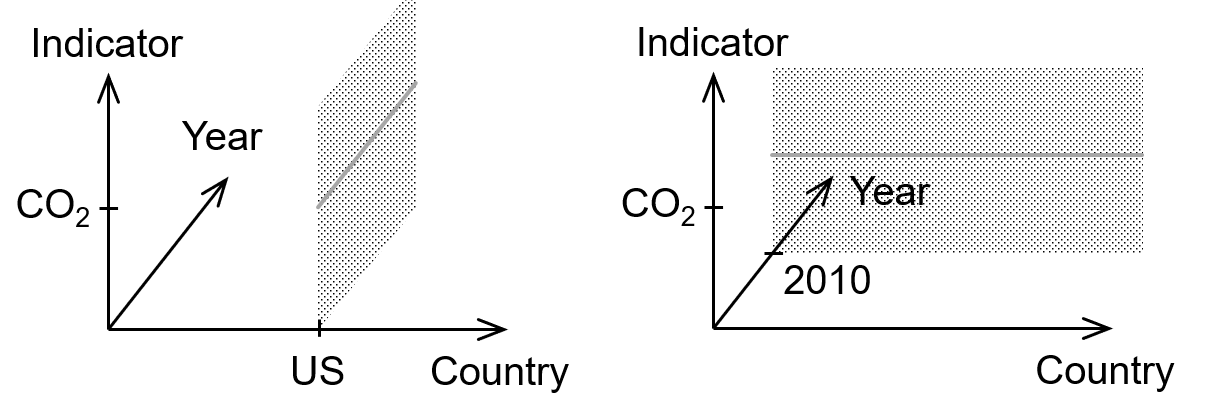
\includegraphics[scale=0.25]{figures/cubetp}
  \vspace{0.5em}
  \caption{The World Bank provider allows users to first choose
    a country or a year and then an indicator.}
  \label{fig:cubetp}
\end{subfigure}
\hfill
\begin{subfigure}[b]{0.45\textwidth}
  \centering
  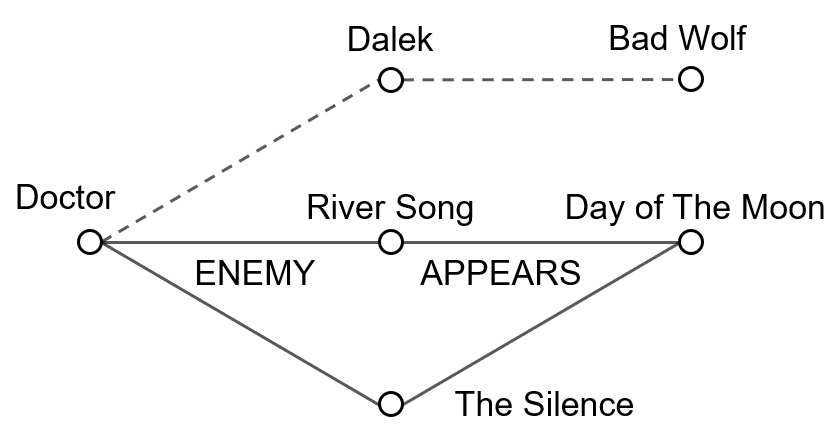
\includegraphics[scale=0.28]{figures/graphtp}
  \caption{The user specifies a path through the data, possibly with
    placeholders to select multiple nodes.}
  \label{fig:graphtp}
\end{subfigure}
\vspace{-0.5em}
\caption{Design of type providers for exploring data cubes and graph databases.}
\label{fig:three graphs}
\end{figure}


\subsubsection*{Graph Database Type Provider}
Our third type provider allows users explore data from graph databases. A graph database
consists of nodes representing entities and relationships between them. In the context of
data journalism, graph databases have been used for example in The Panama Papers reporting \cite{panama}.

The following example explores a database of Doctor Who characters and episodes. It retrieves
all enemies of the Doctor that appear in the Day of the Moon episode:

\begin{thegamma}
drwho.Character.Doctor
  .'ENEMY OF'.'[any]'
  .'APPEARED IN'.'Day of the Moon'
\end{thegamma}

We start from the \ikvd{Doctor} node and then follow two relationships. We use
\ikvd{\textquotesingle ENEMY OF\textquotesingle.\textquotesingle [any]\textquotesingle}
to follow links to all enemies of the Doctor and then specify
\ikvd{\textquotesingle APPEARED IN\textquotesingle.\textquotesingle Day of the Moon\textquotesingle}
to only select only such enemies that appear in a specific episode. The resulting query
is illustrated in Figure~\ref{fig:graphtp}.

The provider works with any graph database and generates members automatically, based on the
data in the database. In the above example, \ikvd{ENEMY OF} and \ikvd{APPEARED IN} are labels
of relations and \ikvd{Doctor} and \ikvd{Day of the Moon} are labels of nodes. The
\ikvd{[any]} member defines a placeholder that can be filled with any node with the specified
relationships. The results returned by the provider is a table of properties of all nodes
along the specified path. As discussed in the next section, such table can be further queried
using the tabular data type provider.

\newpage
% ==================================================================================================

\section{Motivation}
\label{sec:motivation}

The Gamma aims to adapt the recent innovations in programming language research, especially the
work on type providers, into a form where it could be used in practice by journalists and other
non-expert interested in data exploration. We start with a careful consideration of our target
application domain, i.e.~data analyses produced by journalists and citizen data scientists that
are published online. We look at both practical requirements for such programming environment
and requirements arising from our focus on journalism. This analysis is based on the author's
experience of collaborating with journalists\footnote{Citations removed to preserve anonymity.},
review of literature on data journalism, e.g.~\cite{ddj,edcj17,edcj18} and more general trends in
journalism.

\subsection{Open Journalism}
Journalism continually develops and responds to the many challenges it faces \cite{future}.
Two recent challenges are relevant to our work. The first is building trust in media.
One way of establishing trust in the age of fake news is to be more transparent about editorial
decisions, process and original sources.

Many journalists believe that opening up the process
shows the quality and trustworthiness of their work~\cite{transparency}.
The second challenge is reader engagement. To develop a relationship with readers, journalists are
increasingly looking for meaningful ways of engagement. This includes reader comments, involvement
of citizen journalists \cite{comments,citizen} and the development of new interactive formats
\cite{youdraw}. To address the above challenges, a tool for data exploration should satisfy the
following three requirements.

\paragraph{Trust Through Transparency}
To support trustworthiness, data analyses should be transparent. The reader should be able to
determine what is the source of analysed data and how has the data been transformed. As much as
possible, these capabilities should also be accessible to non-expert readers.

\paragraph{Reproducibility for Fact Checking}
It should be possible to re-run the analysis to verify that it produces the presented results.
However, running an opaque script is not enough. A reader should be able to recreate the analysis
by following the necessary steps from the original data source to the end result.

\paragraph{Encouraging Meaningful Engagement}
The tool should support a mechanism through which readers can engage in a meaningful discussion.
For example, it should allow modifying of parameters of a data visualization in order to show
how different choices affect the final result.

\begin{figure}
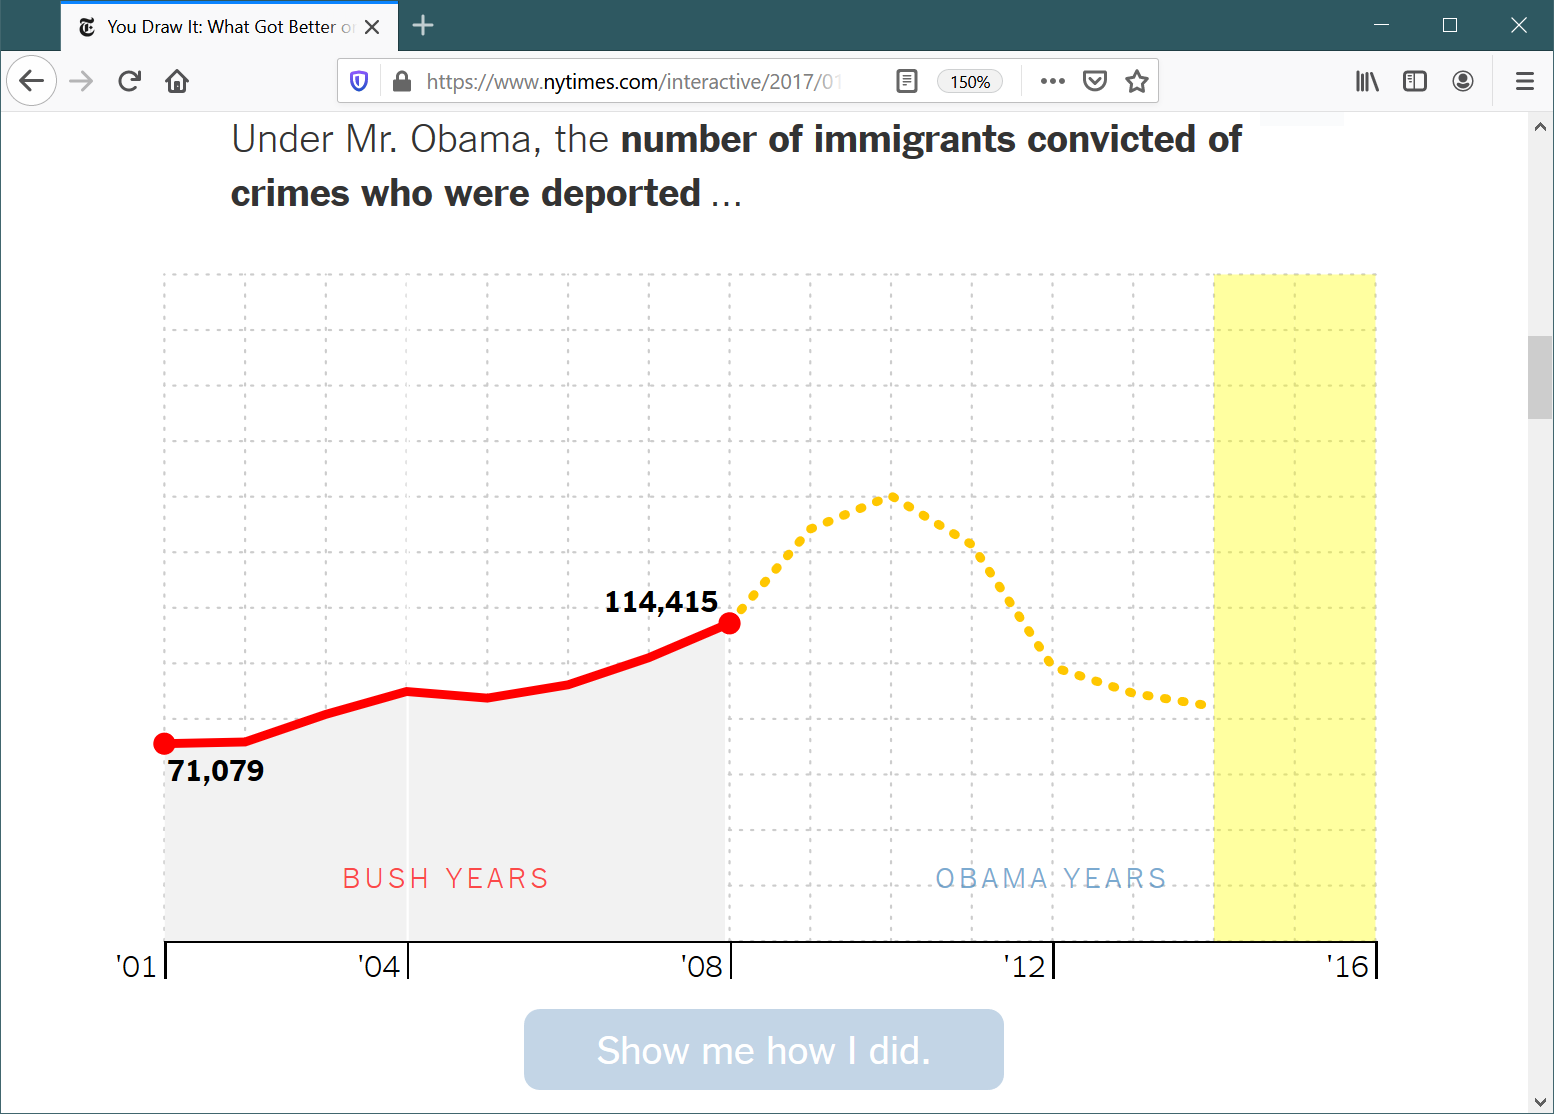
\includegraphics[width=1\columnwidth]{figures/nyt}
\caption{New York Times article on Obama's legacy \cite{youdraw}. The article asks the reader to make a guess
(engagement), but only lists ``Immigration and Customs Enforcement'' as a source of data.}
\label{fig:nyt}
\end{figure}

\subsection{End-user Data Exploration}
Our aim is to make programmatic data exploration accessible to journalists, but we want to keep
the desirable properties of text-based programming. In particular, source code of a data
exploration should provide a full reproducible record of how the data analysis has been done.
As end-users, journalists have a number of interesting characteristics. They work under tight
deadline and data exploration is only a complementary skill. They also need to work with a wide
range of data sources, including big data tables (e.g.~Iraq War documents leak) or graph
databases (e.g.~Panama Papers). This leads to a number of practical requirements on the programming
environment.

\paragraph{Conceptual Simplicity}
We target end-users who cannot dedicate much time to learning about a tool prior
to using it. Consequently, using the tool should require understanding of only a small number
of concepts. Once the user understand a small number of concepts, they should be able to complete
basic data exploration tasks.

\paragraph{Uniformity across Data Sources}
The users should be able to navigate through large databases, query relational databases and
query graph databases through the same mechanism. Ideally, expertise gained with one data source
should also be transferable to working with another data source.

\paragraph{Learning without Experts}
Sarkar \cite{learning} reports that users learn how to use Excel either by talking to experts,
or by seeing a feature in a spreadsheet received from a colleague. In our circumstances, experts
are unlikely to be available, so the tool should support learning from examples. When looking at
a work done and published by another person, the user needs to see (and be able to understand)
how a task was completed.

\begin{figure}
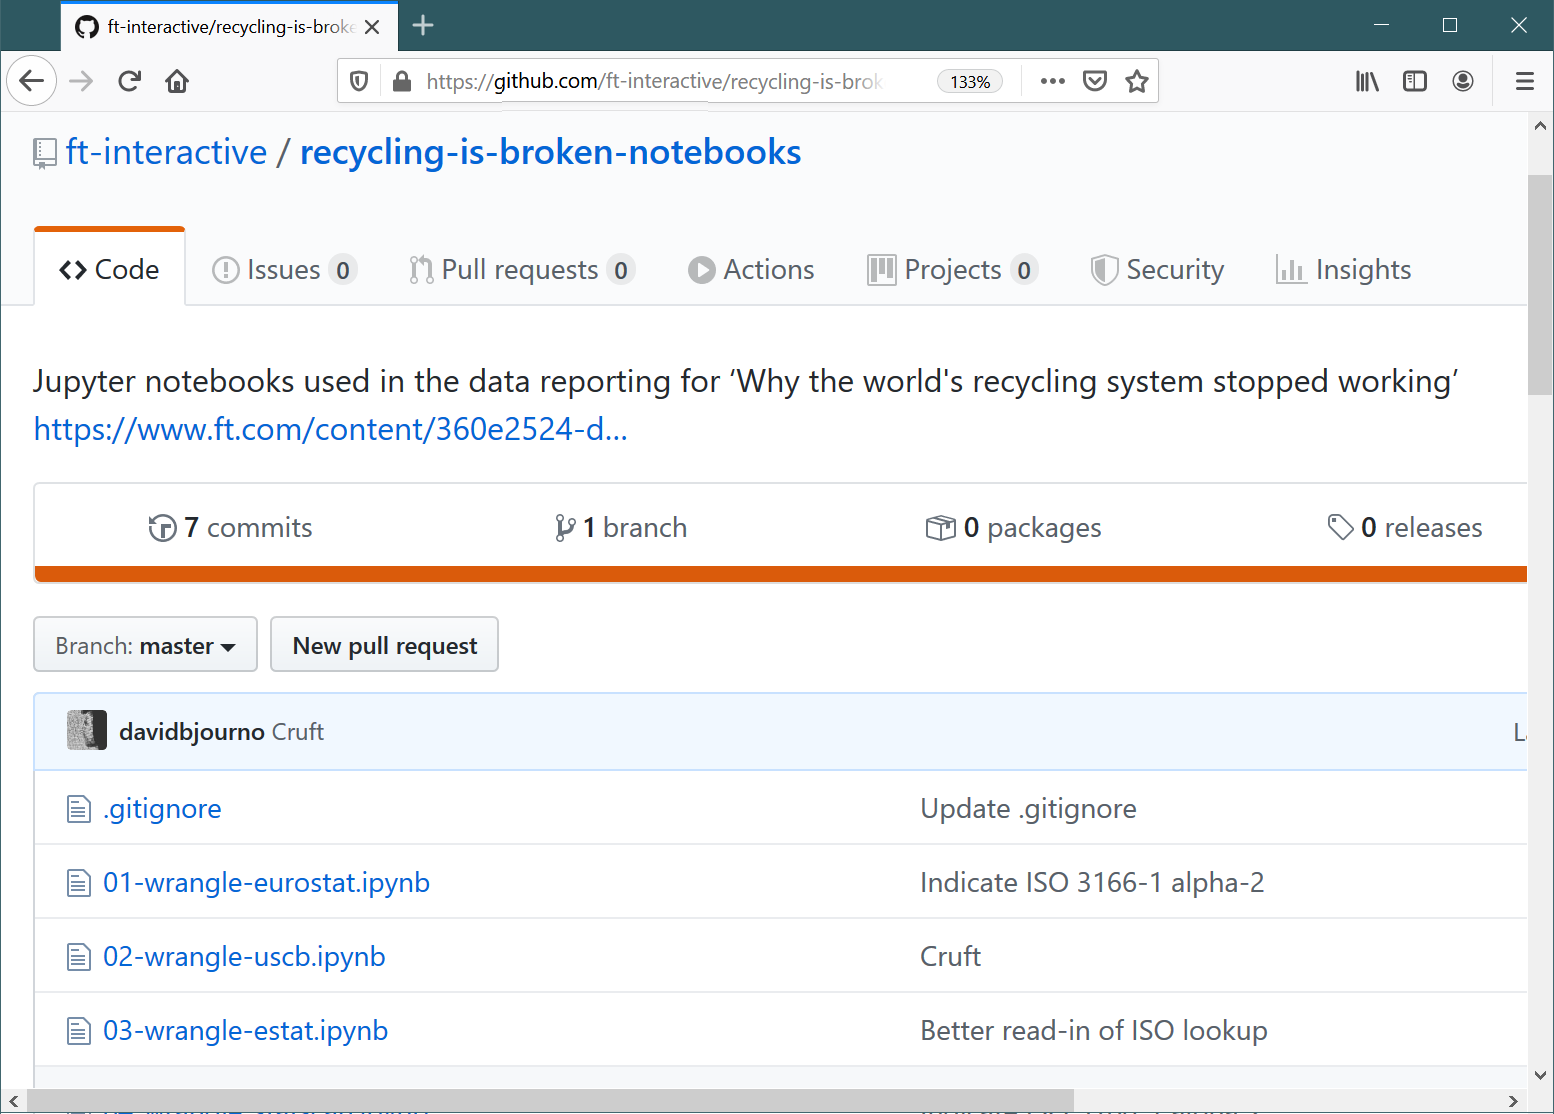
\includegraphics[width=1\columnwidth]{figures/ft}
\caption{Financial Times analysis of recyclable waste. Full source is provided as Jupyter Notebooks
on GitHub \cite{ftnotebooks}, but re-running the analysis is difficult, even for an expert.}
\label{fig:ft}
\end{figure}

% ==================================================================================================



% ==================================================================================================

\section{Design}
\label{sec:design}

We identified a number of requirements for a data exploration tool for journalists earlier.
First, using the tool should result in transparent and reproducible data analyses that can be
understood and modified by non-experts. Second, the tool should minimze the number of concepts
that the user needs to understand and, subsequently, allow them to learn through exploration
and from examples. In this section, we discuss how our design aims to satisfy those requirements.

\subsection{Correct and complete}
any program can be created by autocomplete, all programs created by autocomplete are correct

\subsection{Lowering the Barrier to Entry}
Data exploration tasks, such as querying tables, have a certain irreducible complexity.
Regardless of the interface, the user will be exposed to concepts such as filtering,
sorting and grouping. Our design aims to lower the barrier to entry by stratifying the concepts
into first-level \emph{iterative prompting} principle and second-level \emph{domain specific
languages} for each kind of data source.
The user needs to master the iterative prompting principle in order to start working
with the system. However, using individual data sources can be mastered gradually.

\paragraph{Iterative Prompting}
Iterative prompting is an interaction principle where the user repeatedly invokes an
auto-complete prompt and makes a selection from the offered options. The principle is closely
related to both code completion and the use of command line. Iterative prompting is novel as an
overarching interaction principle for program construction.

In code completion, the auto-complete
prompt is invoked only in certain contexts, e.g.~when accessing a member of an object through a
variable defined earlier in code. It requires the user to be sufficiently familiar with the
programming language in order to get to a point where they are offered a list of members. In
contrast, our system only requires choosing the initial data source. The rest of the programming
is done via iterative prompting. The iterative nature of iterative prompting makes it similar to
using the command line or REPL (read-eval-print-loop) tools. However, those repeatedly ask the
user to type code or commands.

%https://www.nngroup.com/articles/recognition-and-recall/
We argue that iterative prompting is easier than other forms of interaction, because it
follows the \emph{recognition over recall} usability heuristic. The users are only required to
choose from an offered list of options, rather than having to recall a possible command
(to type in a command line) or a syntax in a text-based programming environment.

\paragraph{Domain Specific Languages}
The access to individual data sources in The Gamma is facilitated through a domain specific
language, which defines the primitives that are offered to the user in the auto-complete prompts
invoked through iterative prompting. The domain specific languages are embedded in The Gamma --
they define merely the available members (and specify how to evaluate a chain of members), but
they cannot define any custom syntax.

We discuss the individual domain specific languages for querying data tables, graph databases and
data cubes in a later section. The complexity of those languages differs. The previously discussed
language for querying tabular data is the most complex one. However, The Gamma makes it easy for
the user to start exploring and learning new languages, because they are all accessible via
iterative prompting.

\subsection{Building the Magic Escalator of Knowledge}
As discussed earlier, The Gamma is designed for users who work under tight deadlines and only
analyse data as their secondary task. The Gamma aims to support such users by having a low
barrier for entry and making it easy to learn independently.

\paragraph{Design for Percolation}
When analysing how Excel users learn Sarkar \cite{learning} points out that users learn new
features opportunistically when the usage of a feature is apparent in a spreadsheet. For
example, users can learn different functions to use in formulas, because those are visible in
the cell. Learning how to use a wizard for creating charts in this way is not possible because
it leaves no trace in the spreadsheet -- only the final result. Sarkar's recommendation is to
\emph{design for percolation}, i.e.~in a way where looking at the final result makes it apparent
what feature has been used and how.

\paragraph{Text-based Source Code}
In The Gamma, each step in the iterative prompting process results in an identifier that is
added to the source code. This means that a program constructed solely through iterative prompting
keeps a full trace of how it was created. Seeing the resulting source code provides the user all
information that they need to recreate the program, not just by copying it, but also by using the
iterative prompting mechanism. The Gamma represents code as text and allows the user to edit it
freely, so not all interactions leave a trace. For example, deleting the most recently selected
option and choosing a different one is not apparent from the result.


% ==================================================================================================

\begin{figure}
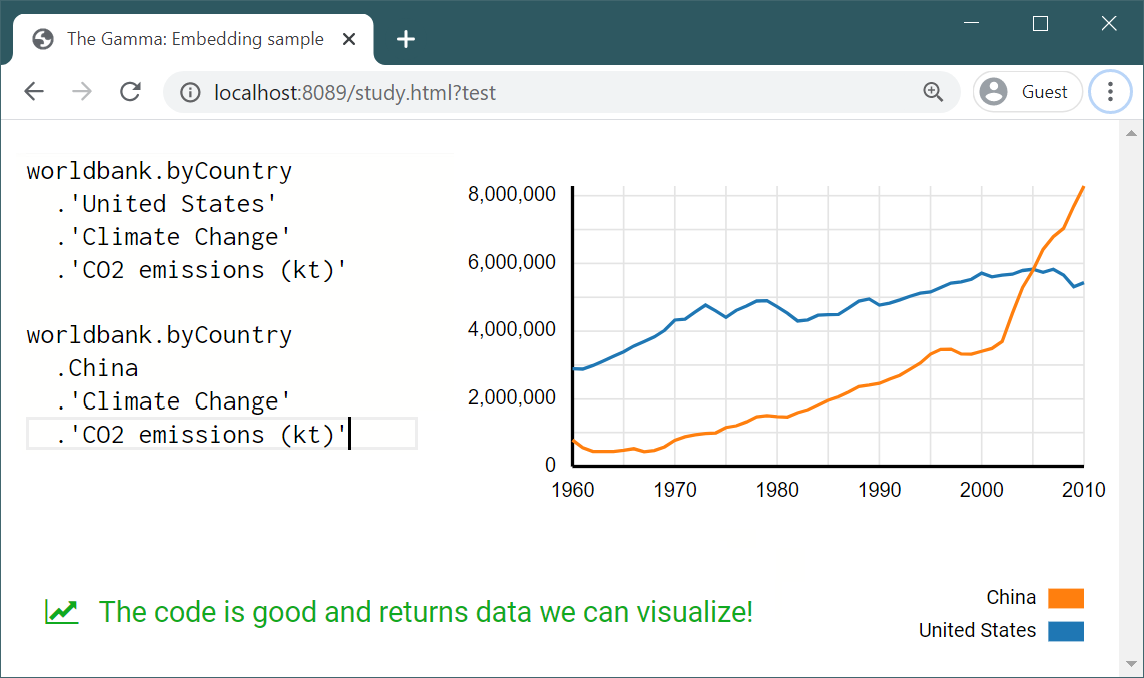
\includegraphics[width=1\columnwidth]{figures/sidebyside}
\caption{The Gamma environment with an automatically generated chart comparing CO2 emissions
of China and United States.}
\label{fig:sidebyside}
\end{figure}


% ==================================================================================================

\section{Use cases}
\label{sec:cases}

The Gamma aims to simplify programmatic data exploration while keeping enough expressive power
to allow users to create interesting data visualizations. We consider the expressive power in
this section and assess simplicity in the next one. We used The Gamma to analyse
the UK government expenditure, activities of a research institute, Olympic medals and
information about the Doctor Who series\footnote{Links removed to preserve anonymity.}.
In this section, we consider two interesting larger examples.

\subsection{If Michael Phelps were a Country}
Michael Phelps has won so many medals that media compared him to
countries.\footnote{\href{https://www.npr.org/sections/thetorch/2016/08/14/489832779/}{\small\bf\ttfamily npr.org/sections/thetorch/2016/08/14/489832779/}}
Using the tabular data provider, we construct a chart shown in Figure~\ref{fig:cases} that
produces a country league table including Michael Phelps:\footnote{Available at: \url{http://gallery.thegamma.net/86/}}

\begin{thegamma}
\kvd{let} data = olympics
    .'group data'.'by Team'.'sum Gold'.then
    .'sort data'.'by Gold descending'.then
    .paging.skip(43).take(4)
    .'get series'.'with key Team'.'and value Gold'

\kvd{let} phelps = olympics
  .'filter data'.'Athlete is'.'Michael Phelps'.then
  .'group data'.'by Athlete'.'sum Gold'.then
  .'get series'.'with key Athlete'.'and value Gold'

charts.bar(data.append(phelps))
  .setColors(["#aec7e8","#aec7e8","#1f77b4"])
\end{thegamma}

The core of the data analysis is done in two commands. The first counts gold medals by countries
and uses paging to fetch 4 countries with suitable number of medals. In the second, we abuse the
grouping operation to aggregate data for just a single group. The two data series are then assigned
to local variables (for readability) and passed to the \ikvd{chart.columns} function.
In this case study, the core data exploration can be constructed via iterative prompting, but
building a chart requires invoking the \ikvd{append} operation and specifying colors using a list.

\subsection{The Most Frequent Doctor Who Villains}
In the second case study, we list Doctor Who villains by the number of episodes in which they
appear.\footnote{Available at: \url{http://gallery.thegamma.net/87/}} This is interesting as it
combines the graph database provider for fetching the data with the tabular data provider for
summarization:

\begin{thegamma}
\kvd{let} topEnemies = drWho.Character.Doctor
  .'ENEMY OF'.'[any]'.'APPEARED IN'.'[any]'.explore
  .'group data'.'by Character name'
    .'count distinct Episode name'.then
  .'sort data'.'by Episode name descending'.then
  .paging.take(8).'get series'
    .'with key Character name'.'and value Episode name'

chart.bar(topEnemies)
\end{thegamma}

Lines 1-2 use the graph database provider to find all paths linking the Doctor node with any
character linked via \ikvd{ENEMY OF}, followed by any episode linked by \ikvd{APPEARED IN}.
This produces a table that can be analysed using the tabular data provider by choosing the
\ikvd{explore} member. For each character (the villain) we count the total number of
distinct episodes in the table. The result is shown in Figure~\ref{fig:cases}.

The logic is not trivial, but it performs a fairly sophisticated data analysis that involves a
graph database query followed by an SQL-like data aggregation. The code can be constructed
using iterative prompting (with the exception of the numbers in paging). It can also be constructed
gradually and instantaneous prviews support the user while doing so.

\begin{figure}
\centering
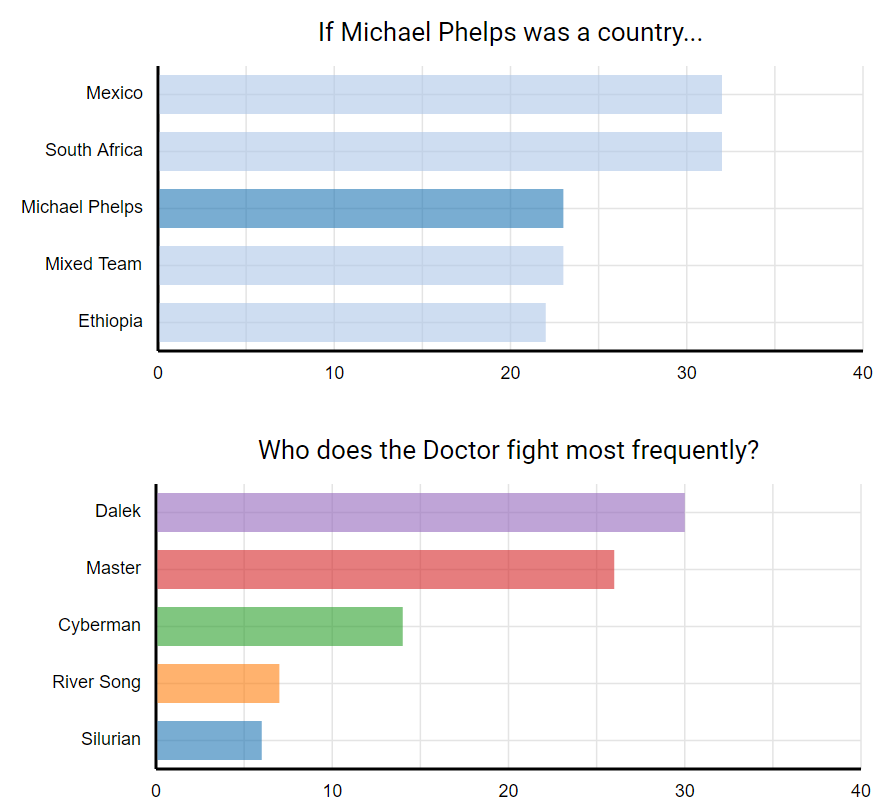
\includegraphics[width=1\columnwidth]{figures/cases}
\caption{Charts produced by two The Gamma case studies.}
\label{fig:cases}
\end{figure}

% ==================================================================================================

\section{User study}
\label{sec:study}

Our goal is to develop an easy-to-learn tool that journalists and other non-programmers can use
for producing transparent data analyses. To evaluate the extent to which The Gamma achieves this,
we conduct a user study. We recruit participants among the operations and business team of a
non-profit research organization and investigate three research questions.

\paragraph{RQ1: Can non-programmers explore data with The Gamma?}
We give participants one of four simple data exploration tasks and see if they can complete the
task using The Gamma and, possibly, how much assistance they need.

\paragraph{RQ2: Can knowledge transfer between data sources?}
Our first hypothesis is that users familiar with the iterative prompting principle will be able to
use an unfamiliar data source. In two of the tasks, participants are shown one data source and
then asked to work with a different one.

\paragraph{RQ3: Can users learn from just code samples?}
Our second hypothesis is that users can learn through percolation, i.e.~by looking at the source
code of published analyses. In one of our tasks, participants are given a code sample, but only a
minimal explanation of The Gamma environment.

\subsection{Study design}
We perform between-subjects study to evaluate the first experience of using The Gamma.
We recruit 13 participants (5 male, 8 female) from a business team
of a research lab working in various non-technical roles (project management,
partnerships, communications) including one former journalist.

We split participants into 4 groups. We first gave a brief 5 minute demonstration of The
Gamma and then asked participants to complete a task. Finally, we conducted a short semi-structured
group interview and later sent participants a follow-up questionnaire. The four tasks were:

\begin{itemize}
\item \emph{Expenditure.} Participants were given a demo using \emph{worldbank}.
  They were asked to use the \emph{expenditure} data source to compare the UK government spending
  on ``Public order and safety'' and ``Defence'' in terms of GDP.
\item \emph{Lodrs.} Participants were given a demo using \emph{worldbank}.
  They were asked to use the \emph{lords} data source (a table with House of Lords
  members expenses) to find a members representing London with the highest travel costs.
\item \emph{Worldbank.} Participants were given a minimal explanation of The Gamma environment and
  a code sample using \emph{worldbank}. They were asked to solve a different task using
  the \emph{worldbank} data source.
\item \emph{Olympics.} Participnts were given a demo using \emph{olympics}.
  They were asked to solve a more complex problem using the same data source.
\end{itemize}

We let participants work independently, but offered guidance if they got stuck for longer period of
time. Tasks \emph{expenditure} and \emph{lords} aim to answer the questions RQ1 and RQ2; the task
\emph{worldbank} aims to answer RQ1 and RQ3. In \emph{olympics}, we test RQ1 using a more complex
data source and we ask further questions to explore their understanding of the data source.

\begin{table}
  \centering
  \begin{tabular}{l l l c l}
    \toprule
      & {\small \textit{Task}}
      & {\small \textit{Kind}} & {\small \textit{Done}}
      & {\small \textit{Notes}} \\
    \midrule
    \small \#1 & \small expenditure & \small cube & \priority{50} & {\small Obtained one of two data series}\\
    \small \#2 & \small expenditure & \small cube & \priority{100} & {\small Explored furhter data series }\\
    \small \#3 & \small expenditure & \small cube & \priority{100}& {\small Explored further data series }\\
    \small \#4 & \small expenditure & \small cube & \priority{75}& {\small With hint to use another member }\\
    \small \#5 & \small expenditure & \small cube & \priority{100}& {\small Explored further data series }\\
    \small \#6 & \small worldbank & \small cube & \priority{75} & {\small With general syntax hint }\\
    \small \#7 & \small worldbank & \small cube & \priority{100} & {\small Completed very quickly }\\
    \small \#8 & \small worldbank & \small cube & \priority{100} & {\small Extra time to find data }\\
    \small \#9 & \small lords & \small table & \priority{75} & {\small  Struggled with composition}\\
    \small \#10 & \small lords & \small table & \priority{100} & {\small Completed very quickly }\\
    \small \#11 & \small lords & \small table & \priority{75} & {\small With a hint to avoid operations}\\
    \small \#12 & \small olympics & \small table & \priority{75}  & {\small With a hint to avoid operations}\\
    \small \#13 & \small olympics & \small table & \priority{75}  & {\small Hints about `then' and operations}\\
    \bottomrule
  \end{tabular}
  \caption{Overview of the work completed by individual participants. The marks denote:
    \priorityc{75} = required some guidance, \priorityc{50} = partially completed.}
  \label{tab:tasks}
  \vspace{-1em}
\end{table}

\subsection{Results}
Table~\ref{tab:tasks} summarizes the work done by the study participants.
For each participant, we record the task, the kind of data source used in the task and the
level of completion. For participants who needed assistance, the notes section details the help
given. We analyse the hints in the next section. Table~\ref{tab:quest} shows the results of the
follow-up questionnaire.

\paragraph{RQ1: Can non-programmers explore data with The Gamma?}
Three results allow us to answer RQ1 in the affirmative. First, 7 out of 9
participants agree or strongly agree that they ``found the system easy to use''. Second,
participants spent between 10 and 25 minutes (average 17 minutes) working with The Gamma and
all 12 out of 13 participants completed the task; 6 participants required some assistance,
but 3 of those faced one issue (discussed later) that could be covered in the introductory
presentation. Third, a number of participants shared positive comments in the semi-structured
interview.

Participant \#3 found the system simple, but also points out an issue about data provenance,
which we discuss later:

\begin{quote}
\emph{``This is actually pretty simple to use. You think about the logic of what you're actually
  asking and then you try to get it into the format you can. But knowing where it comes from
  would tell you how to trust it.''}
\end{quote}

Similarly, participant \#2, notes that The Gamma alleviated their unease about code:

\begin{quote}
\emph{``For somebody who does not do coding or programming, this does not feel that daunting.
  It's not like you're giving me large screen full of code, which is reassurring.''}
\end{quote}

Finally, participant \#5 suggested the system could be used as an educational tool for teaching
critical thinking with data. They answer a follow-up question about what training materials would
the students need as follows:

\begin{quote}
\emph{``I don't think they'd need more than 5 minute video (..) this is the data
  source, this is what's in there.''}
\end{quote}

\paragraph{RQ2: Can knowledge transfer between data sources?}
Our study does not conclusively answer RQ2. There is some evidence in favor of a positive answer.
In the practical part, two of the tasks (\emph{expenditure} and \emph{lords}) used a different data
source in the introductory presentation than the one that the participants were asked to use.
Participants were able to complete those tasks, although \emph{lords} has been more challenging
as it involves a more complex data source. In the interview, participant \#2 also gives a positive
answer:

\begin{quote}
\emph{``I found it quite easy to translate what you showed us in the demo to the new dataset.
   I though it was quite easy to just get how that works.''}
\end{quote}

Negative evidence is offered by the follow-up questionnaire. When asked
whether they would know how to approach a task using a new data source, 5 out of 9 participants
diagree or strongly disagree that they would know how to approach it without any further guidance.
Participants did not believe that knowledge can easily transfer to another
data source.

\paragraph{RQ3: Can users learn from just code samples?}
A positive answer to RQ3 is supported by the \emph{worldbank} task results, the follow-up questionnaire
and interview comments. In the task, participants were given only a
minimal demo of the iterative prompting principle together with print-out of 2 code samples.
All three were able to complete a related task using the same data source. In the follow-up
questionnaire, only 2 out of 9 participants disagree or strongly disagree that
they would know how to approach a task using an unfamiliar data source when given ``a number
of code samples''.

In the semi-structured interview, participants were asked what would be the most useful format
of educational material about The Gamma (code samples, video tutorials, etc.).
Participant \#7 noted that \emph{``a video would just be this [i.e.~a code sample] anyway''}, while
participant \#13 (former journalist) answered:

\begin{quote}
  \emph{``I think providing one video of one example is good and maybe a couple of little examples
  of code wher people can see the kind of things you can do.''}
\end{quote}

This is aligned with our design goal. Once the user understands the iterative prompting principle
(which can be done through a video tutorial), they can learn how to use any specific data source
just from code samples.

\subsection{Further observations}
In this section, we briefly discuss a number of observations about The Gamma design that
emerged from the study, some of which suggest ways of improving the system.

\paragraph{Making complex things possible may hurt}
As discussed earlier, The Gamma language supports operations such as \ikvd{take(5)}. Most type
providers never generate those, but the provider for working with tabular data is an exception.
When filtering data, the provider allows specifying a condition on numerical attributes such as
\ikvd{olympics.\textquotesingle filter data\textquotesingle.\textquotesingle Year is greater than\textquotesingle(2004)}.

Three participants (\#11, \#12, \#13) struggled to complete a task, because they
initially attempted to use those operations. However, those violate the iterative prompting
principle as one cannot type `.' after \ikvd{\textquotesingle Year is greater than\textquotesingle}.
This suggests that we should avoid operations in type providers for data access, even if it
limits the expressive power of the type provider.

\paragraph{Benefits and drawbacks of text}
The Gamma is based on text to aid transparency. Text hints that there is no hidden state and
the reader sees the full code. The study suggests that using a text editor has both
benefits and drawbacks compared to alternatives such as structured editors~\cite{structure-based,livenut,lamdu}.
Most participants had no difficulty navigating around source code, making edits or deleting code
fragments, which is arguably harder in an unfamiliar structured editor.

We observed two issues in the study. Participant \#2 struggled with correct indentation, starting a second command
with more indentation than needed and participant \#6 had a syntax error in an unrelated command,
which prevents charts from rendering. Some participants used the text editor effectively,
e.g.~participant \#5, who used copy-and-paste to fetch the same data series for multiple countries.

\begin{table}
  \centering
  \begin{tabular}{p{19em} c c}
    \toprule
      {\small \textit{Questionnaire item}} & {\small \textit{Avg}} & {\small \textit{Sdv}} \\
    \midrule
    \small Considering your experience \& possible use of The Gamma:\\
    \small \quad I found the system easy to use. & \small 2.11 & \small 0.87\\
    \small \quad Journalists will be able to use it to analyse data. & \small 2.67 & \small 1.05\\
    \small \quad Readers will be able to critically examine the analyses. & \small 2.44 & \small 0.68\\
    \small Thinking about the usability of the system:\\
    \small \quad The resulting programs are easy to understand. & \small 2.33 & \small 0.82\\
    \small \quad The text editor for creating them was easy to use. & \small 2.33 & \small 0.94\\
    \small \quad Finding the right item in the auto-complete was easy. & \small 2.56 & \small 1.42\\
    \small I would know how to approach a task using a new data source\\
    \small \quad If given a comprehensive video tutorial. & \small 2.00 & \small 1.24\\
    \small \quad If given a number of code samples. & \small 2.78 & \small 1.13\\
    \small \quad Without any further guidance. & \small 3.56 & \small 1.17\\
    \bottomrule
  \end{tabular}
  \caption{Summary of follow-up questionnaire responses using
    a 5-point Likert scale (1 = strongly agree, 5 = strongly disagree) over 9 subjects.}
  \label{tab:quest}
\end{table}

\paragraph{How users understand the `then' member}
When interviewing participants who worked with a tabular data source, we
asked about their understanding of the \ikvd{then} member. This is a regular member generated by the
type provider (i.e.~not a keyword), but it has a special meaning. Consider
the following example which calculates the average travel expenses and total number of
representatives per county using the UK House of Lords expenses data:

\begin{thegamma}
expneses.'group data'.'by County'
  .'average Travel Costs'.'count distinct Name'.then
\end{thegamma}

The \ikvd{then} member is used to complete a part of a query where the user can continue
adding items to build a list. Here, we select two aggregations to be calculated for each
county before choosing \ikvd{then} and applying other operations such as sorting.

Two participants (\#12 and \#13) initially thought that \ikvd{then} is used to split a command
over multiple lines, but rejected the idea after experimenting and noting that they can insert
line breaks elsewhere. One correctly concluded that it ``allows us to chain together the
operations'' of the query. Participant \#13 needed a hint about using the
\ikvd{then} member and later reflected:

\begin{quote}
  \emph{``When you explained about the `dot then' that was a really useful thing to know.
  When I found that, I was like this is fine, this is doable. If I knew this from the start,
  it would [have been easier].''}
\end{quote}

This comment summarizes an important fact. Although iterative prompting allows the users to start
exploring new data sources, the domain specific languages used by more complex data sources have
their own design principles that users need to understand to use the data source effectively.

\subsection{Study conclusions}
The motivation behind The Gamma is to make simple programmatic data exploration accessible to
journalists and other non-experts. Main-stream programming languages have the benefit of
reproducibility and transparency, but are difficult to use. Our study shows that non-experts
are able to solve basic data exploration tasks using The Gamma. When asked whether The Gamma
is something that journalists could learn how to use, participant \#13 (a former journalist) answered:

\begin{quote}
\emph{``Yeah, I think so. There's a lot of effort going into data journalism that
  programming could make much quicker, but I was always nervous about code. (...)
  Something like this would really simplify things.''}
\end{quote}

The Gamma is based on the iterative prompting principle which lowers the barrier to entry, but
it is worth noting that it does not fully eliminate complexity involved in data querying.
Instead, it provides a way of structuring the complexity. Iterative prompting makes it easy to
get started, but complex data sources will inevitably require additional learning. The Gamma
makes this easier by allowing users to learn from published code samples.

% ==================================================================================================

\section{Discussion}
We design a programming environment that can make programmatic data exploration accessible
to journalists. This is aligned with recent developments in journalism, which aims to build
trust through transparency and greater reproducibility as well as provide meaningful ways of
engagement.

\subsection{Evaluating The Gamma}
Data exploration environments are complex systems that do not yield to simple controlled
experimentation. We evaluate The Gamma using criteria inspired by Olsen~\cite{evaluating}.

\begin{itemize}
\item \emph{Importance.} Open journalism has the potential to make factual claims backed by
data more commonplace and enable wider audience engage with such claims. As such, we contribute
towards solving an important societal issue.

\item \emph{Expressive leverage.} The Gamma reduces the number of concepts that the user needs
to master to just the \emph{iterative prompting} principle, although complex data sources may
add more concepts through their domain specific languages.

\item \emph{Empowering new participants.} As demonstrated by our user study, The Gamma allows
non-experts, including those not comfortable with code, to perform basic programmatic
data exploration tasks.

\item \emph{Generality.} Finally, our case studies show that The Gamma can be used to solve
a wide range of data manipulation tasks involving many data sources including tabular data,
data cubes and graph databases.
\end{itemize}

\subsection{Remaining design issues}
There remain a number of aspects of data exploration in the context of journalism that
The Gamma does not address. Two of those, data provenance and data availability were also
observed by the participants in our study.

\paragraph{Data provenance}
Data sources such as \ikvd{olympics} or \ikvd{worldbank} are defined when initializing The Gamma
programming environment, but the system does not currently show where such data comes from.
For some data sources, the source is e.g.~a CSV file published by the government. In this case,
we can easily show the source. However, other type providers may pre-process data. Displaying
data source in such cases would require more sophisticated provenance tracking \cite{provenance}.

\paragraph{Data availability}
In the current version, The Gamma does not have a way of informing the user what data sources
are available. In other words, the user needs to know the first identifier, such as \ikvd{olympics},
to get started. We could address this by choosing a data source as the first step of iterative
prompting and perhaps typing \ikvd{.olympics}. However, a more fundamental issue is finding
the data source in the first place. This could be partly addressed by a type provider for a
currated online database such as Enigma Public\footnote{\url{https://docs.enigma.com/public}}.
Providing access to open government data repositories such as \href{http://data.gov.uk}{\small\bf\ttfamily data.gov.uk}
is more appealing, but very challenging due to their unstructured nature.

\subsection{Evaluation limitations}
The evaluation conducted in this paper is qualitative and exploratory in nature. In particular,
we do not make any quantitative claims about the usability of The Gamma and its learning curve.
Our study also focused on the core iterative prompting interaction, but our case studies often
required using other features such as operations with parameters.

Although The Gamma is open-source, it has not been deployed in production in a newsroom so far.
This would lead to valuable insights, but it requires finding a suitable fortuitous opportunity.
Finally, we also do not compare the usability of The Gamma with the usability of other popular
systems such as Tableau \cite{tableau}. It would be possible to set tasks that can be completed
in both systems, but the systems have very different aims making such comparison problematic.

\section{Conclusions}
We present The Gamma, a simple data exploration environment. The Gamma is motivated by the needs
of journalists working with data, who need to produce transparent and easy-to-understand reports
backed by data that are transparent and engaging, all the while facing tight deadlines.

The Gamma is based on a single interaction principle, \emph{iterative prompting}, can be used to
complete a wide range of data exploration tasks using a variety of data sources including tabular
data, data cubes and graph databases. The design lowers the barrier to entry for programmatic
data exploration and it makes it easy to learn the system independently from examples and by
experimentation.

% \section{Acknowledgments}
% Yo

% BALANCE COLUMNS
\balance{}

% REFERENCES FORMAT
% References must be the same font size as other body text.
\bibliographystyle{ACM-Reference-Format}
\bibliography{paper}


\end{document}

%%% Local Variables:
%%% mode: latex
%%% TeX-master: t
%%% End:
